% Diese Datei ist Teil des Buchs "Schreibe Dein Programm!"
% Das Buch ist lizensiert unter der Creative-Commons-Lizenz
% "Namensnennung - Weitergabe unter gleichen Bedingungen 4.0 International (CC BY-SA 4.0)"
% https://creativecommons.org/licenses/by-sa/4.0/deed.de

\chapter{Bäume}
\label{cha:trees}

\index{Baum}Bäume sind eine Form von Daten, die (wie Listen) besonders
oft in der Informatik vorkommt.  Oft ergeben sich baumförmige
Datendefinitionen aus der Problemstellung.  Wenn wir über diese
Datendefinitionen abstrahieren, entsteht eine universell verwendbare
Form von Daten, der \textit{Binärbaum}\index{Binärbaum}.  Diese
Binärbäume sind ähnlich vielseitig wie Listen und erlauben uns
außerdem, Daten so in Bäumen zu organisieren, dass wir sie schnell
wiederfinden können.

\section{Stammbäume}

Die Idee, den Baum als Metapher für eine bestimmte Form von Daten zu
benutzen, findet sich bereits in der Bibel, die Wörter wie
"<Baumstumpf"> und "<Spross"> benutzt, um Abstammmung zu beschreiben.
Erste bildliche Darstellungen von Stammbäumen sind aus diesen
Beschreibungen ab dem 11.\ Jahrhundert abgeleitet worden.

Das Stammbaum-Beispiel ist etwas ausgetreten, aber dennoch instruktiv.
In Stammbäumen sind in der Regel für eine Person ihr Name sowie
Verbindungen zu den beiden Eltern vermerkt.  Das führt zu folgender
Datendefinition.
%
\begin{lstlisting}
; Eine Person hat folgende Eigenschaften:
; - Name
; - Elternteil #1
; - Elternteil #2
\end{lstlisting}
%
Diese Definition lässt offen, um was für Daten es sich bei den beiden
Elternteilen handelt.  Natürlich sind es auch Personen, aber wenn wir
in einem Stammbaum weit genug nach oben gehen, sind diese irgendwann
unbekannt: Jeder konkrete Stammbaum endet irgendwo.  Wir brauchen also
auch noch eine Repräsentation für einen "<unbekannten Elternteil">
ohne (bekannte) Eigenschaften:
%
\begin{lstlisting}
; Ein unbekannter Elternteil hat keine Eigenschaften
(define-record unknown-parent
  make-unknown-parent
  unknown-parent?)
\end{lstlisting}
%
Daraus entsteht eine Datendefinition für "<Elternteil">:
%
\begin{lstlisting}
; Ein Elternteil ist eins der folgenden:
; - eine Person
; - ein unbekannter Elternteil
\end{lstlisting}
%
Diese~-- und die Datendefinition für "<Person"> können wir nun in Code
übersetzen:
%
\begin{lstlisting}
(define-record person
  make-person
  person?
  (person-name string)
  (person-parent-1 parent)
  (person-parent-2 parent))

(define parent
  (signature
   (mixed person unknown-parent)))
\end{lstlisting}
%
Für das unbekannte Elternteil stellen wir gleich mal einen Wert her:
%
\begin{lstlisting}
(define an-unknown-parent (make-unknown-parent))
\end{lstlisting}
%
Hier ein kleiner Stammbaum als Beispiel:
%
\begin{lstlisting}
(define slash
  (make-person "Slash"
               (make-person "Ola Hudson"
                            an-unknown-parent
                            an-unknown-parent)
               (make-person "Anthony Hudson"
                            an-unknown-parent
                            an-unknown-parent)))
(define london-hudson
  (make-person "London Hudson"
               slash
               (make-person "Perla Ferrar"
                            an-unknown-parent
                            an-unknown-parent)))
\end{lstlisting}
%
Wir schreiben nun eine Funktion, die feststellen soll, ob jemand der
Vorfahr einer Person ist, so etwa:
%
\begin{lstlisting}
; Ist jemand Vorfahr:in einer Person?
(: ancestor? (string person -> boolean))

(check-expect (ancestor? "Slash" london-hudson) #t)
(check-expect (ancestor? "Axl" london-hudson) #f)
\end{lstlisting}
%
Die Schablone für diese Funktion sieht folgendermaßen aus:
%
\begin{lstlisting}
(define ancestor?
  (lambda (name person)
    ...
    (person-name person)
    (person-parent-1 person)
    (person-parent-2 person)
    ...))
\end{lstlisting}
%
Was können wir mit diesen Bestandteilen anfangen?  Den Namen der
Person könnten wir mit dem gesuchten Namen vergleichen~-- wenn ja,
handelt es sich um einen Vorfahren:
%
\begin{lstlisting}
(define ancestor?
  (lambda (name person)
    (if (string=? name (person-name person))
        #t
        ...)
    (person-parent-1 person)
    (person-parent-2 person)
    ...))
\end{lstlisting}
%
Bei \lstinline{(person-parent-1 person)} und
\lstinline{(person-parent-2 person)} handelt es sich um gemischte
Daten.  Wir könnten die nötige Verzweigung direkt in
\lstinline{ancestor?} einbauen.  Genauso können wir eine separate
Funktion schreiben, welche die Frage beantwortet, ob ein Elternteil
Vorfahr ist.  Da es zwei Elternteile gibt, lohnt sich tendenziell eine
solche separate Funktion mit Kurzbeschreibung und Signatur wie folgt:
%
\begin{lstlisting}
; Ist jemand Vorfahr:in eines Elternteils?
(: parent-ancestor? (string parent -> boolean))
\end{lstlisting}
%
Diese Funktion schreiben wir gleich im Anschluss.  Aber ihre Signatur
ist genug, damit wir die Schablone in Funktion \lstinline{ancestor?}
weiter ausfüllen, indem wir überprüfen, ob Elternteil Nr.~1 oder Nr.~2
Vorfahr ist:
%
\begin{lstlisting}
(define ancestor?
  (lambda (name person)
    (if (string=? name (person-name person))
        #t
        (if (or (parent-ancestor? name (person-parent-1 person))
                (parent-ancestor? name (person-parent-2 person)))
            #t
            #f))))
\end{lstlisting}
%
Diese Funktion ist schon korrekt, aber sie könnte noch etwas eleganter
sein.  Der zweite \lstinline{if}-Ausdruck liefert \lstinline{#t}, falls
die Bedingung \lstinline{#t} und \lstinline{#f}, falls die Bedingung
\lstinline{#f} liefert: Es kommt also immer das Ergebnis der Bedingung
heraus.  Das ist eine allgemein anwendbare Regel:
%
\begin{lstlisting}
(if $b$ #t #f) $=$ $b$
\end{lstlisting}
%
Wir können \lstinline{ancestor?} also verkürzen auf:
%
\begin{lstlisting}
(define ancestor?
  (lambda (name person)
    (if (string=? name (person-name person))
        #t
        (or (parent-ancestor? name (person-parent-1 person))
            (parent-ancestor? name (person-parent-2 person))))))
\end{lstlisting}
%
Auch den verbleibenden \lstinline{if}-Ausdruck können wir noch
loswerden, weil er \lstinline{#t} ergibt, wenn die Bedingung
\lstinline{#t} ergibt oder wenn der \lstinline{or}-Ausdruck
\lstinline{#t} liefert.  Wir können deshalb die Funktion mit einem
großen \lstinline{or} schreiben:
%
\begin{lstlisting}
(define ancestor?
  (lambda (name person)
    (or (string=? name (person-name person))
        (parent-ancestor? name (person-parent-1 person))
        (parent-ancestor? name (person-parent-2 person)))))
\end{lstlisting}
%
Notwendig war diese Vereinfachung nicht, aber schöner sieht das
Resultat schon aus, finden wir!

Es fehlt noch die Hilfsfunktion \lstinline{parent-ancestor?}.  Hier
sind ein paar Tests:
%
\begin{lstlisting}
(check-expect (parent-ancestor? "Slash" london-hudson) #t)
(check-expect (parent-ancestor? "Axl" london-hudson) #f)
(check-expect (parent-ancestor? "Slash" an-unknown-parent) #f)
\end{lstlisting}
%
Gerüst und Schablone ergeben sich~-- wie immer~-- aus der
Datendefinition von \lstinline{parent}:
%
\begin{lstlisting}
(define parent-ancestor?
  (lambda (name parent)
    (cond
      ((person? parent) ...)
      ((unknown-parent? parent) ...))))
\end{lstlisting}
%
Für den ersten Fall können wir \lstinline{ancestor?} benutzen, im
zweiten Fall können wir mit \lstinline{#f} antworten:
%
\begin{lstlisting}
(define parent-ancestor?
  (lambda (name parent)
    (cond
      ((person? parent)
       (ancestor? name parent))
      ((unknown-parent? parent)
       #f))))
\end{lstlisting}
%
Fertig!

\begin{aufgabeinline}
  Ändere die Funktion \lstinline{ancestor?} dahingehend, dass eine
  Person nicht ihr eigener Vorfahr ist.
  Achte darauf, dass ansonsten die Funktion noch richtig arbeitet!
  Wird die Funktion einfacher?
\end{aufgabeinline}

\section{Binärbäume}
\label{sec:trees}

Wir schauen uns nochmal die Record-Defininiton von \lstinline{person}
an:
%
\begin{lstlisting}
(define-record person
  make-person
  person?
  (person-name string)
  (person-parent-1 parent)
  (person-parent-2 parent))
\end{lstlisting}
%
Vielleicht hat Dich das an eine Record-Definition aus
Kapitel~\ref{cha:selbstbezug} erinnert:
%
\begin{lstlisting}
(define-record confluence
  make-confluence
  confluence?
  (confluence-location  string)
  (confluence-main-stem river)
  (confluence-tributary river))
\end{lstlisting}
%
Die Struktur ist bei beiden Definitionen gleich.  Insbesondere
enthalten beide Definitionen jeweils zwei Selbstreferenzen.  Bei
\lstinline{person} ist die Selbstreferenz auf \lstinline{parent}, das
so definiert ist:
%
\begin{lstlisting}
(define parent
  (signature
   (mixed person unknown-parent)))
\end{lstlisting}
% 
Bei \lstinline{confluence} ist die Selbstreferenz auf
\lstinline{river}:
%
\begin{lstlisting}
(define river
  (signature (mixed creek confluence)))
\end{lstlisting}
%
Die jeweils anderen Fälle von \lstinline{parent} und
\lstinline{person} unterscheiden sich leicht:
%
\begin{lstlisting}
(define-record unknown-parent
  make-unknown-parent
  unknown-parent?)

(define-record creek
  make-creek
  creek?
  (creek-origin string))
\end{lstlisting}
%
In beiden steckt selbst aber keine Selbstreferenz mehr.  Beide
Datendefinitionen bilden baumartige Strukturen ab: Ein
\lstinline{person}- oder \lstinline{confluence}-Record bildet einen
Ast, der zweifach verzweigt.  Ein Baum endet jeweils bei
\lstinline{unknown-parent}- oder \lstinline{creek}-Records.  Weil die
"<inneren"> Äste immer zweifach verzweigen, handelt es sich in beiden
Fällen um \textit{Binärbäume}\index{Binärbaum}.  

Über diese beiden Sätze von Definitionen können wir abstrahieren.
Fangen wir mit \lstinline{person} und \lstinline{confluence} an.  Der
gängige Name für die Verzweigungen innerhalb eines Binärbaums ist
\textit{Knoten}\index{Knoten} oder \textit{innerer Knoten}, auf
Englisch \textit{node}.  Wir brauchen außerdem einen Namen für die
"<Namensdaten">, die bei beiden noch dabei sind.  Üblich ist
\textit{Markierung}\index{Markierung}, auf Englisch \textit{label}.
Die Signatur für den Selbstbezug nennen wir einfach \lstinline{tree}:
%
\begin{lstlisting}
(define-record node
  make-node node?
  (node-label string)
  (node-left-branch tree)
  (node-right-branch tree))
\end{lstlisting}
%
Das Wort "<branch"> heißt wörtlich übersetzt "<Zweig">, wir verwenden
aber die Begriffe "<linker Teilbaum"> und "<rechter Teilbaum">, was im
Deutschen üblicher ist.\index{Teilbaum}

Bei der Definition für \lstinline{tree} brauchen wir noch einen Namen
für die Werte an den Rändern des Baums~-- genannt
\textit{Blätter}\index{Blatt}, auf Englisch \textit{leaf}.
%
\begin{lstlisting}
(define tree
  (signature (mixed leaf node)))
\end{lstlisting}
%
Es fehlt noch die Definition von \lstinline{leaf}.  Hier ist es nicht
ganz so einfach, weil \lstinline{creek} noch einen Namen enthält,
\lstinline{unknown-parent} aber nicht.  Wir müssen also über beide
abstrahieren.  Einen Namen haben wir ja schon~-- \lstinline{leaf}~--
es fehlt noch das \lstinline{lambda}:
%
\begin{lstlisting}
(define tree-of
  (lambda (leaf)
    (signature (mixed leaf node))))
\end{lstlisting}
%
Das zieht noch eine weitere Änderung nach sich, weil \lstinline{tree}
ja in der Definition von \lstinline{node} verwendet wird.  Wir müssen
da entsprechend den \lstinline{leaf}-Parameter mit durchziehen:
%
\begin{lstlisting}
(define-record (node-of leaf)
  make-node node?
  (node-label string)
  (node-left-branch (tree-of leaf))
  (node-right-branch (tree-of leaf)))
\end{lstlisting}
%
Die Notation für die Abstraktion der Record-Signatur mit den
Extra-Klammern um \lstinline{(node-of leaf)} haben wir bisher erst
einmal gesehen, bei der Definition von \lstinline{cons-list-of} in
Abschnitt~\ref{function:cons-list-of} auf Seite~\pageref{function:cons-list-of}.

Wir könnten an dieser Stelle fertig sein.  Wir nehmen aber noch eine
Verallgemeinerung vor: Wie wir sehen werden, müssen die Markierungen
in Bäumen nicht unbedingt Zeichenketten sein~-- wir werden da noch
andere Arten von Werten ablegen wollen.  Darum abstrahieren wir auch
über die Signatur der Markierungen noch.  Außerdem reichen wir noch
die Datendefinitionen nach:
%
\begin{lstlisting}
; Ein Knoten besteht aus
; - Markierung
; - linken Ast
; - rechter Ast
(define-record (node-of leaf label)
  make-node node?
  (node-label label)
  (node-left-branch (tree-of leaf label))
  (node-right-branch (tree-of leaf label)))

; Ein Binärbaum ist entweder ein Blatt oder ein Knoten
(define tree-of
  (lambda (leaf node-label)
    (signature (mixed leaf (node-of leaf node-label)))))
\end{lstlisting}
%
Das nun ist die Definition eines Binärbaums in Reinform.  Hier sind
zwei Beispiele, bei denen wir einfach den Wert \lstinline{#f} als
Blatt verwendet haben:
%
\begin{lstlisting}
(: tree1 (tree-of false number))
(define tree1 (make-node 3 (make-node 4 #f (make-node 7 #f #f)) #f))
(: tree2 (tree-of false number))
(define tree2 (make-node 17 (make-node 3 #f tree1) #f))
\end{lstlisting}
%
Hier ist noch ein weiteres Beispiel, bei dem die Blätter Zahlen sind
und die Markierungen Zeichenketten
\begin{lstlisting}
(: tree3 (tree-of number string))
(define tree3 (make-node "Axl"
                         (make-node "Slash" 17 
                                            (make-node "Duff" 14 23))
                         12))
\end{lstlisting}
%
% FIXME: Bild mit tree1, tree2, tree3 - dabei auch Begriff Wurzel einführen
Wir können \lstinline{tree-of} benutzen, um die Definition von
\lstinline{river} und \lstinline{parent} zu vereinfachen:
%
\begin{lstlisting}
(define river (tree-of creek string))
(define river? node?)
(define make-confluence make-node)
(define confluence-location node-label)
(define confluence-main-stem node-left-branch)
(define confluence-tributary node-right-branch)
\end{lstlisting}
%
\begin{aufgabeinline}
  Definiere \lstinline{person} mit Hilfe von \lstinline{tree-of}!
\end{aufgabeinline}
%
Auf Bäumen kann man alle möglichen Sachen berechnen.  Ein Beispiel ist
die \textit{Tiefe}\index{Tiefe!eines Baums}, also die maximale Anzahl
Knoten auf dem Weg zu einem Blatt.  (Manchmal heißt diese Größe auch
die \textit{Höhe}\index{Höhe!eines Baums} eines Baums.)  Für die Tiefe
des Baums sind die Signaturen der Blätter und Markierungen egal:
%
\begin{lstlisting}
; Tiefe eines Baums berechnen
(: depth ((tree-of %leaf %label) -> natural))
\end{lstlisting}
%
Hier sind zwei Testfälle:
%
\begin{lstlisting}
(check-expect (depth tree1) 3)
(check-expect (depth tree2) 5)
\end{lstlisting}
%
Bei \lstinline{tree1} sind es die Knoten mit den Markierunen 3, 4 und
7, die den maximal langen Weg zu einem Blatt bilden.  Bei
\lstinline{tree2} sind es 17, 3, 3, 4, 7.

Es geht wieder los mit der Konstruktionsanleitung.  Wir brauchen die
Schablone für gemischte Daten als Eingabe.  Da die Datendefinition für
Binärbäume zwei Fälle hat, brauchen wir ein \lstinline{cond} mit zwei
Zweigen.  Beim ersten können wir Bedingungen mit \lstinline{node?}
bilden.  Die Blätter haben kein festes Prädikat, aber das sind einfach
alle Bäume, die keine Knoten sind~-- wir können also statt einer
Bedingung \lstinline{else} schreiben:
%
\begin{lstlisting}
(define depth
  (lambda (tree)
    (cond
      ((node? tree) ...)
      (else ... 0))))
\end{lstlisting}
%
In den Knoten stecken zwei Selbstbezüge, wir brauchen also zwei
rekursive Aufrufe:
%
\begin{lstlisting}
(define depth
  (lambda (tree)
    (cond
      ((node? tree)
       ...
       (depth (node-left-branch tree))
       (depth (node-right-branch tree))
       ...)
      (else ...))))
\end{lstlisting}
%
Für die Tiefe zählt nur der Weg mit der maximalen Anzahl von Knoten.
Außerdem müssen wir den Knoten in \lstinline{tree} noch mitzählen.
Blätter zählen überhaupt nicht:
%
\begin{lstlisting}
(define depth
  (lambda (tree)
    (cond
      ((node? tree)
       (+ 1
          (max (depth (node-left-branch tree))
               (depth (node-right-branch tree)))))
      (else 0))))
\end{lstlisting}
%
Fertig!
%
\begin{aufgabeinline}
  Schreiben Sie eine Funktion, die alle Knoten eines Baums zählt!
\end{aufgabeinline}

\section{Bäume für's Suchen}
\label{sec:search-trees}

Viele Probleme bei der Programmierung sind "<Suchprobleme">: Einen
Namen, eine Telefonummer, eine Bestellnummer aus einer Liste
heraussuchen.  Darum geht es in diesem Abschnitt und wir fangen damit
an, dass wir das Wort "<Liste"> wörtlich nehmen und eine Funktion wie
folgt schreiben:
%
\begin{lstlisting}
; ist Wert Element einer Liste?
(: member? (%a (list-of %a) -> boolean))
\end{lstlisting}
%
Wir haben eine Signaturvariable verwendet, weil es sich bei den
Listenelementen mal um Zahlen, mal um Zeichenketten, mal um etwas
anderes handeln kann.  Hier sind ein paar Testfälle:
%
\begin{lstlisting}
(check-expect (member? 5 empty) #f)
(check-expect (member? 2 (list 1 2 3)) #t)
(check-expect (member? "Slash" (list "Axl" "Slash")) #t)
(check-expect (member? "Buckethead" (list "Axl" "Slash")) #f)
\end{lstlisting}
%
Hier Gerüst und Schablone für Funktionen auf Listen:
%
\begin{lstlisting}
(define member?
  (lambda (element list)
    (cond
      ((empty? list) ...)
      ((cons? list)
       ... 
       (first list)
       (member? element (rest list))
       ...))))
\end{lstlisting}
%
Bei der leeren Liste kann die Funktion nur \lstinline{#f}
zurückgeben.  Bei der Cons-Liste legt die Schablone nahe, dass die
Funktion erst einmal prüfen sollte, ob \lstinline{(first list)} das
gesucht Element ist.

Klingt einfach, oder?  Aber \emph{wie} prüfen wir das?  Wir könnten
das hier hinschreiben:
%
\begin{lstlisting}
(= element (first list))
\end{lstlisting}
%
\ldots~aber das würde die Funktion auf Zahlen beschränken, weil
\lstinline{=} nur auf Zahlen funktioniert.  Für die beiden Testfälle
mit Zeichenketten müssten wir \lstinline{string=?} verwenden.  Wir
müssen also \lstinline{member?} über \lstinline{=} respektive
\lstinline{string=?} abstrahieren, noch bevor die Funktion überhaupt
fertig ist.  Wir brauchen wie immer einen weiteren Parameter und
nennen ihn \lstinline{equals?}:
%
\begin{lstlisting}
(define member?
  (lambda (equals? element list)
    (cond
      ((empty? list) ...)
      ((cons? list)
       ... 
       (first list)
       (member? equals? element (rest list))
       ...))))
\end{lstlisting}
%
(Aufpassen: Der rekursive Aufruf muss~-- wie immer~-- auch durch den
neuen Parameter erweitert werden.)

Jetzt können wir den Vergleich mit Hilfe von \lstinline{equals?}
durchführen und diesen mit einer binären Verzweigung verarbeiten:
%
\begin{lstlisting}
(define member?
  (lambda (equals? element list)
    (cond
      ((empty? list) #f)
      ((cons? list)
       (if (equals? element (first list))
           #t
           (member? equals? element (rest list)))))))
\end{lstlisting}
%
Signatur und Testfälle haben von dem neuen Parameter noch nichts
mitbekommen.  Die \lstinline{equals?}-Funktion akzeptiert zwei
Listenelemente und liefert ein boolesches Ergebnis.  Da die
Listenelemente die Signatur \lstinline{%a}
haben, sieht die Signaturdeklaration für \lstinline{member?} so aus:
%
\begin{lstlisting}
(: member? ((%a %a -> boolean) %a (list-of %a) -> boolean))
\end{lstlisting}
%
Bei den Testfällen müssen wir jeweils noch die richtige
Vergleichsfunktion übergeben.  Das ist \lstinline{=} für Zahlen und
\lstinline{equals?} für Zeichenketten.
%
\begin{lstlisting}
(check-expect (member? = 5 empty) #f)
(check-expect (member? = 2 (list 1 2 3)) #t)
(check-expect (member? string=? "Slash" (list "Axl" "Slash")) #t)
(check-expect (member? string=? "Buckethead" (list "Axl" "Slash")) #f)
\end{lstlisting}
%
Fertig!

Allerdings hat \lstinline{member?} einen Nachteil: Bei kurzen Listen
oder wenn das gesuchte Element am Anfang der Liste steht, wird
\lstinline{member?} ziemlich schnell fertig.  Aber stell Dir vor, die
Liste hat ein paar Millionen Elemente und das gesuchte Element ist am
Ende.  Oder gar nicht drin: Dann muss \lstinline{member?} die gesamte
Liste abklappern.
%
\begin{aufgabeinline}
  Schreibe mit Hilfe von \lstinline{member?} eine Funktion, die von
  zwei Listen alle Elemente liefert, die in beiden Listen stehen, also
  deren Schnittmenge.  Wie lange braucht diese Funktion im
  ungünstigsten Fall?
\end{aufgabeinline}
%
Kann irgendwie schneller herausfinden, ob ein Wert Element einer Menge
ist oder nicht?  In der Tat ist das möglich, aber nicht mit Listen:
Wir brauchen eine andere Struktur, um das Suchen zu beschleunigen~--
Bäume.

\begin{figure}[tb]
\begin{tikzpicture}[level/.style={sibling distance=60mm/#1}]
\node (z){$M$}
  child {node (a) {$B$}
    child {node (b) {$A$}
      child {node {$\bullet$}} 
      child {node {$\bullet$}}
    }
    child {node (g) {$D$}
      child {node {$\bullet$}}
      child {node {$\bullet$}}
    }
  }
  child {node (j) {$O$}
    child {node (k) {$N$}
      child {node {$\bullet$}}
      child {node {$\bullet$}}
    }
    child {node (l) {$R$}
      child {node {$\bullet$}}
      child {node {$\bullet$}}
    }
  };
\end{tikzpicture}
  \caption{Sortierter Baum über Buchstaben}
  \label{fig:searchtree}
\end{figure}

Schau Dir mal Abbildung~\ref{fig:searchtree} an.  In diesem Baum musst
Du nicht alle Elemente anschauen, um ein bestimmtes Element zu
finden.  Das liegt daran, dass die Buchstaben in dem Baum auf
bestimmte Art nach dem Alphabet sortiert sind:

Die Wurzel mit der Markierung $M$ hat zwei Teilbäume~-- die
Markierungen des linken Teilbaums liegen allesamt \emph{vor} $M$ im
Alphabet, alle Markierungen des rechten Teilbaums \emph{nach} $M$.
Wenn Du also nach einem Buchstaben suchst~-- nehmen wir mal $D$~--
dann weißt Du, wenn Du die Wurzel mit $M$ siehst, dass $D$ im linken
Teilbaum von $M$~-- mit der Markierung $B$ und von da aus im rechten
Teilbaum von $B$ stehen muss.  Die Knoten $A$, $O$, $N$, $R$ kannst Du
ignorieren.

Die Suche braucht also höchstens so viele Schritte wie der Baum tief
ist.  Das ist schonmal besser, als in der Liste zu suchen, wo wir
potenziell alle Elemente anschauen müssen.

Programmieren wir das also!

Wir fangen mit einem sortierten Baum über reellen Zahlen an.
(Reelle Zahlen deshalb, weil wir sie einfach mit \lstinline{=} und
\lstinline{<} vergleichen können.  Wir verallgemeinern das später.)
Die Zahlen kleben als Markierungen an den Knoten.  An den Blättern
steht nichts relevantes, wir benutzen deshalb immer \lstinline{#f}.
Entsprechend sehen Kurzbeschreibung und Signatur so aus:
%
\begin{lstlisting}
; Ist eine Zahl in einem sortierten Baum vorhanden? 
(: tree-member? (real (tree-of false real) -> boolean))
\end{lstlisting}
%
Die Signatur \lstinline{false}\index{false@\texttt{false}} ist neu:
Sie beschreibt nur den Wert \lstinline{#f}.  Entsprechend gibt es
natürlich auch eine Signatur
\lstinline{true}\index{true@\texttt{true}} für \lstinline{#t}.

Als Beispielbaum für die Tests benutzen wir diesen hier:
%
\begin{lstlisting}
(define tree4
   (make-node 5
              (make-node 3 #f #f)
              (make-node 17
                         (make-node 10 #f (make-node 12 #f #f))
                         #f)))
\end{lstlisting}
%
Hier sind ein paar Tests:
%
\begin{lstlisting}
(check-expect (tree-member? 5 tree4) #t)
(check-expect (tree-member? 17 tree4) #t)
(check-expect (tree-member? 3 tree4) #t)
(check-expect (tree-member? 10 tree4) #t)
(check-expect (tree-member? 2 tree4) #f)
\end{lstlisting}
%
Hier ist das Gerüst:
\begin{lstlisting}
(define tree-member?
  (lambda (value tree)
    ...))
\end{lstlisting}
%
In die Schablone für Bäume tragen wir gleich den zweiten Fall ein:
Wenn die Funktion ein Blatt erreicht, dann ist das \lstinline{value}
definitiv nicht im Baum, das Ergebnis dann \lstinline{#f}:
%
\begin{lstlisting}
(define tree-member?
  (lambda (value tree)
    (cond
      ((node? tree)
       ...
       (node-label tree)
       (tree-member? value (node-left-branch tree))
       (tree-member? value (node-right-branch tree))
       ...
      (else #f)))))
\end{lstlisting}
%
Bei Knoten können wir drei Fälle unterscheiden: Wenn die Markierung
gerade das gesucht \lstinline{value} ist, wenn \lstinline{value}
kleiner ist als die Markierung (also im linken Teilbaum stehen muss)
und wenn sie größer ist.  Daraus ergibt sich folgende
Weiterentwicklung:
\begin{lstlisting}
(define tree-member?
  (lambda (value tree)
    (cond
      ((node? tree)
      ...
      (tree-member? value (node-left-branch tree)))
      (tree-member? value (node-right-branch tree))
      ...
      (cond
         ((= value (node-label tree)) #t)
         ((< value (node-label tree)) ...
         (else ...)))
      (else #f))))
\end{lstlisting}
%
Da \lstinline{(node-label tree)} zweimal vorkommt, machen wir dafür
eien Definition und setzen die Bestandteile der Schablone so zusammen:
%
\begin{lstlisting}
(define tree-member?
  (lambda (value tree)
    (cond
      ((node? tree)
       (define label (node-label tree))
       (cond
         ((= value label) #t)
         ((< value label)
          (tree-member? value (node-left-branch tree)))
         (else
          (tree-member? value (node-right-branch tree)))))
      (else #f))))
\end{lstlisting}
%
Fertig!

\section{Sortierte Bäume herstellen}

In den Testfällen für \lstinline{tree-member?} haben wir immer den
Baum \lstinline{tree4} vwerwendet, den wir direkt mit
\lstinline{make-node} konstruiert haben.  Dabei mussten wir selbst
darauf achten, dass er auch sortiert ist.  In diesem Abschnitt
automatisieren wir diese Konstruktion, dann kann dabei auch kein
Fehler passieren.  (Wenn wir korrekt programmieren zumindest.)

Wir schreiben dafür eine Funktion, die ein neues Element in einen
bestehenden sortierten Baum einfügt.  Kurzbeschreibung und Signatur
sind wie folgt:
%
\begin{lstlisting}
; Zahl in sortierten Baum einfügen 
(: tree-insert (real (tree-of false real) -> (tree-of false real)))
\end{lstlisting}
%
Testfälle brauchen wir als nächstes.  Wir könnten das so machen wie
immer: Wir schreiben einen Aufruf von \lstinline{tree-member?} hin und
den Ergebniswert, den wir uns erhoffen.  In diesem Fall aber ist es
gar nicht so wichtig, was der Ergebniswert genau ist.  Wichtig ist,
dass ein eingefügtes Element im Ergebnisbaum auch drin ist.  Außerdem
ist es mühsam, immer den ganzen Baum hinzuschreiben.  Darum benutzen
wir \lstinline{tree-member?}, um \lstinline{tree-insert} zu testen.
%
\begin{lstlisting}
(check-expect (tree-member? 5 (tree-insert 5 tree4)) #t)
(check-expect (tree-member? 11 (tree-insert 11 tree4)) #t)
\end{lstlisting}
%
Später werden wir feststellen, dass \lstinline{tree-insert}
unterschiedliche sortierte Bäume liefern kann, die allesamt korrekt
sind.
%
\begin{aufgabeinline}
  Die beiden Tests erwarten jeweils, dass \lstinline{#t} bei
  \lstinline{tree-member?} herauskommt.  Wäre es sinnvoll, auch noch
  welche mit \lstinline{#f} zu schreiben?
\end{aufgabeinline}
%
Wenn Du ein mulmiges Gefühl bei den spärlichen beiden Tests hast:
richtig!  In Kapitel~\ref{cha:properties} auf
Seite~\pageref{cha:properties} werden wir zeigen, wie man Funktionen
wie \lstinline{tree-insert} besser testet.

Aber jetzt geht's erst einmal mit der Funktion selbst los.  Gerüst und
Schablone sind genau wie bei \lstinline{tree-member?}:
%
\begin{lstlisting}
(define tree-insert
  (lambda (value tree)
    (cond
      ((node? tree)
        ...
        (tree-insert value (node-left-branch tree))
        (tree-insert value (node-right-branch tree))
        ...)
      (else ...))))
\end{lstlisting}
%
Die Fallunterscheidung bei Knoten ist ebenfalls wie in
\lstinline{tree-member?}, darum können wir auch die Verzweigung aus
der dortigen Schablone übernehmen:
%
\begin{lstlisting}
(define tree-insert
  (lambda (value tree)
    (cond
      ((node? tree)
        ...
        (tree-insert value (node-left-branch tree))
        (tree-insert value (node-right-branch tree))
        ...
        (cond
         ((= value (node-label tree)) ...)
         ((< value (node-label tree)) ...)
         (else ...)))
      (else ...))))
\end{lstlisting}
%
Auch hier ist der erste Fal einfach: Wenn \lstinline{value} gerade die
Markierung eines Knotens ist, dann enthält der Baum den Wert bereits,
die Funktion muss nichts einfügen und kann einfach \lstinline{tree}
liefern.  Auch für den Fall, dass \lstinline{tree} ein Blatt ist (das
letzte \lstinline{else}), ist es recht einfach: Wir konstruieren einen
neuen, einelementigen Baum:
%
\begin{lstlisting}
(define tree-insert
  (lambda (value tree)
    (cond
      ((node? tree)
        ...
        (tree-insert value (node-left-branch tree))
        (tree-insert value (node-right-branch tree))
        ...
        (cond
         ((= value (node-label tree)) tree)
         ((< value (node-label tree)) ...)
         (else ...)))
      (else (make-node value #f #f)))))
\end{lstlisting}
%
Es bleiben noch zwei Fälle, in denen der einzufügende Wert links
beziehungsweise rechts von der Knotenmarkierung liegt.  Er muss
entsprechend im linken oder rechten Teilbaum eingefügt werden: Genau
das erledigen die beiden rekursiven Aufrufe aus der Schablone.  Der
jeweils andere Teilbaum bleibt so wie er ist:
%
\begin{lstlisting}
(define tree-insert
  (lambda (value tree)
    (cond
      ((node? tree)
       (cond
         ((= value (node-label tree)) tree)
         ((< value (node-label tree))
          (make-node (node-label tree)
                     (tree-insert value (node-left-branch tree))
                     (node-right-branch tree)))
         (else
          (make-node (node-label tree)
                     (node-left-branch tree)
                     (tree-insert value (node-right-branch tree))))))
      (else
       (make-node value #f #f)))))
\end{lstlisting}
%
Fertig!

\section{Suchbäume}

Unsere Funktionen \lstinline{tree-member?} und \lstinline{tree-insert}
funktionieren nur auf Zahlen. Die Bäume aus den
Abbildungen~\ref{fig:searchtree} und \ref{fig:degenerated-searchtree}
enthalten aber beide Buchstaben.  Wenn wir andere Werte als Zahlen
zulassen wollen, müssen wir wieder einmal abstrahieren über alles, was
mit Zahlen zu tun hat.

Schau Dir nochmal die Definition von \lstinline{tree-member?} an: Es
gibt zwei Stellen, die "<zahlenspezifisch"> sind, nämlich
\lstinline{=} und \lstinline{<}.  Wenn Zeichenketten in einem
sortierten Baum unterbringen wollten, müssten wir da
\lstinline{string=?} und \lstinline{string<?} hinschreiben.

\begin{aufgabeinline}
  Abstrahiere \lstinline{tree-member?} und \lstinline{tree-insert}
  über \lstinline{=} und \lstinline{<}.

  Übergib mal statt \lstinline{<} die Funktion \lstinline{>}.
  Funktionieren \lstinline{tree-member?} und \lstinline{tree-insert}
  dann noch korrekt?  Wie unterscheiden sich die Bäume, die mit
  \lstinline{<} aus \lstinline{tree-insert} herauskommen von denen mit
  \lstinline{>}?
\end{aufgabeinline}

Die abstrahierten Versionen von \lstinline{tree-member?} und
\lstinline{tree-insert} haben einen Nachteil: Bei jedem Aufruf dieser
Funktionen müssen wir die beiden Argumente für \lstinline{=} und
\lstinline{<} hinschreiben.  Das nervt und ist jedesmal eine
Gelegenheit für einen Fehler, weil wir das vollkommen konsistent
machen müssen.

Wir wollen also versuchen, ohne diese zusätzlichen Parameter
auszukommen.  Das bedeutet aber, dass die Funktionen für \lstinline{=}
und \lstinline{<} in einem der schon vorher existierenden Argumente
unterkommen müssen: \lstinline{value} und \lstinline{tree}.  Wir
machen das mit \lstinline{tree}, weil die benutzen Funktionen
bestimmen, wie der Baum aussehen muss.  Die Idee ist, dass wir die
beiden Funktionen zusammen mit dem Baum "<einpacken">.

FIXME


\section{Sortierte Bäume sind effizienter als Listen}
  
Intuitiv ist die Idee mit dem sortierten Baum beim Suchen
effizienter.  Aber hält diese Intuition auch einer mathematischen
Untersuchung stand?  Betrachte dazu den Baum in "<Ebenen"> --
erste Ebene ist die Wurzel, die zweite Ebene deren Teilbäume, die
dritte Ebene wiederum deren Teilbäume undsoweiter.  Dann passen in
jede Ebene doppelt soviele Knoten wie in die Ebene darüber.

In einen Baum der Tiefe 1 passt auch nur $1 = 2^0$ Knoten, in einen
der Tiefe 2 passen $2^0 + 2^1 = 1+2 = 3$ Knoten, dann 7, dann 15
undsoweiter.  Dir fällt vielleicht auf, dass die Zahlen 1, 3, 7, 15
allesamt Vorgänger einer Zweierpotenz sind.  Wir können deshalb
versuchen, das zu einer Formel zu verallgemeinern.  Die Tiefe des
Baums heißt dabei $t$.  Dann nehmen wir an (oder hoffen zumindest),
dass für für alle 
%
\begin{displaymath}
  2^0 + ... + 2^{t-1} = \sum_{i=0}^{i=t-1} 2^i  = 2^t-1
\end{displaymath}
%
Da es sich bei $t$ um eine natürliche Zahl handelt, können wir
vollständige Induktion anwenden nach der Anleitung in
Abschnitt~\ref{sec:nat-induction-ka} auf
Seite~\pageref{sec:nat-induction-ka}.

Wir müssen also beweisen, dass für alle $t\in\mathbb{N}$ gilt:
%
\begin{displaymath}
  \sum_{i=0}^{i=t-1} 2^i  = 2^t-1
\end{displaymath}
%
$t=0$:
%
\begin{displaymath}
  \sum_{i=0}^{i=0-1} 2^i = 2^0 - 1
\end{displaymath}
%
Beweis:
%
\begin{eqnarray*}
  \sum_{i=0}^{i=-1} 2^i
  &=& 0\\
  &=& 1-1\\
  &=& 2^0 - 1
\end{eqnarray*}
%
(Vielleicht kommt Dir komisch vor, dass die Summe von $0$ bis $-1$
läuft.  Da es keine Zahl zwischen $0$ bis $-1$ gibt, ist die Summe
leer und deshalb das neutrale Element bezüglich der Addition.)

\smallskip

\noindent Induktionsvoraussetzung:
\begin{displaymath}
  \sum_{i=0}^{i=t-1} 2^i  = 2^t-1
\end{displaymath}
%
Induktionsschluss (zu zeigen):
%
\begin{displaymath}
    \sum_{i=0}^{i=(t+1)-1} 2^t = 2^{t+1} - 1
\end{displaymath}
%
Beweis:
%
\begin{eqnarray*}
  \sum_{i=0}^{i=(t+1)-1} 2^i
  &=& \sum_{i=0}^{i=t} 2^i\\
  &=& \sum_{i=0}^{i=t-1} 2^i + 2^t\\
  &=& 2^t-1 + 2^t \quad\textrm{Induktionsvoraussetzung}\\
  &=& 2^t\cdot 2 - 1\\
  &=& 2^{t+1} - 1
\end{eqnarray*}
%
Wozu ist diese Formel gut, fragst Du Dich vielleicht.  Nun, die rechte
Seite können wir umdrehen.  (Bei der linken Seite ist das
schwieriger.) Wenn die Anzahl der Knoten $k$ ist, dann gilt:
%
\begin{displaymath}
  \begin{array}{lrcl}
    & k &=& 2^t - 1\\
    \Longleftrightarrow & k + 1 &=& 2^t\\
    \Longleftrightarrow & \log_2(k+1) &=& t
  \end{array}
\end{displaymath}
%
Die $\log_2$ ist der sogenannte
\textit{Logarithmus}\index{Logarithmus} zur Basis 2, auch genannte
\textit{Zweierlogarithmus}\index{Zweierlogarithmus}.  Das ist die
Umkehrfunktion zur Exponentialfunktion mit der Basis 2.

\begin{figure}[tb]
  \centering
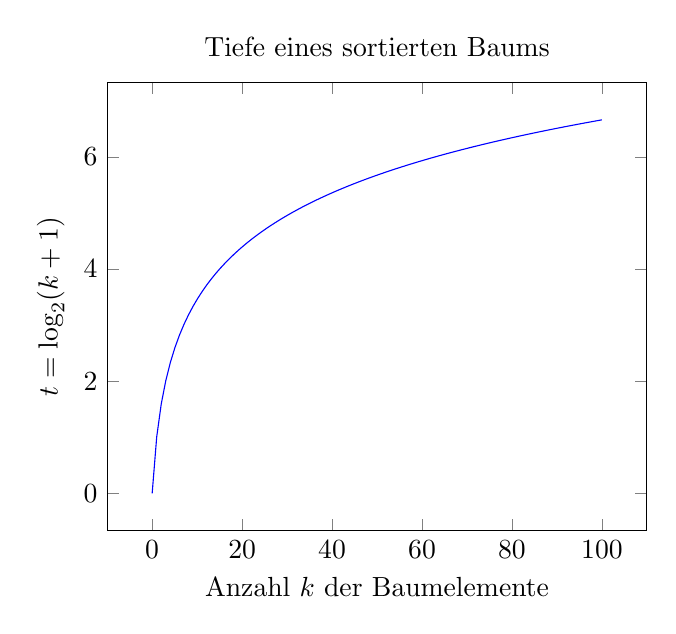
\begin{tikzpicture}
  \begin{axis}[
    title={Tiefe eines sortierten Baums },
    xlabel={Anzahl $k$ der Baumelemente},
    ylabel={$t = \log_2(k+1)$}
    ]
    \addplot [
    blue,
    domain=0:100,
    samples=100,
    ]
    {log2(x+1)}; 
  \end{axis}
\end{tikzpicture}
  \caption{Beziehung zwischen Anzahl von Knoten und Tiefe eines Binärbaums}
  \label{fig:log2}
\end{figure}

Schau Dir Abbildung~\ref{fig:log2} an: Da siehst Du, dass die Tiefe~--
mithin der Logarithmus~-- viel langsamer wächst als die Anzahl der
Knoten, und die Kurve immer flacher wird.  Diese Kurve erklärt, warum
das mit dem sortierten Baum eine gute Idee ist: Die Tiefe des Baums ist ja
die Anzahl der Elemente des Baums, die man abklappern muss, um das
gewünschte Element zu finden.  (Beziehungsweise herauszubekommen, dass
es nicht im Suchbaum ist.)  Das gilt allerdings nur, wenn der Suchbaum
"<voll besetzt"> ist.  Wir müssen uns also irgendwann Gedanken machen,
wie wir dafür sorgen, dass Suchbäume immer möglichst voll besetzt
sind.  Dazu kommen wir später.

\section{Suchbäume konstruieren}

FIXME

\begin{figure}[tb]
\begin{tikzpicture}[level/.style={sibling distance=60mm/#1}]
\node (z){$A$}
    child {node {$\bullet$}}
    child {node (b) {$B$}
      child {node {$\bullet$}}
      child {node (d) {$D$}
        child {node {$\bullet$}}
        child {node (m) {$M$}
          child {node {$\bullet$}}
          child {node (n) {$N$}
            child {node {$\bullet$}}
            child {node (o) {$O$}
              child {node {$\bullet$}}
              child {node (r) {$R$}
                child {node {$\bullet$}}
                child {node {$\bullet$}}
              }
            }
          }
        }
      }
  };
\end{tikzpicture}
  \caption{Entarteter Suchbaum}
  \label{fig:degenerated-searchtree}
\end{figure}

Abbildung~\ref{fig:degenerated-searchtree} zeigt einen Suchbaum, der
nicht voll besetzt ist~-- einen sogenannten \textit{entarteten
  Suchbaum}\index{entarteter Suchbaum}\index{Suchbaum!entartet}. Bei
diesem Suchbaum dauert die Suche genau so lang wie in einer Liste.

\section{Interessantere Suchbäume}


FIXME: Ab hier alt


Für Suchbäume wird ein neuer Record-Typ
definiert.\index{search-tree@\texttt{search-tree}} Zu einem Suchbaum
gehören neben dem Baum selbst auch noch Operationen für
Gleichheit und die "<Kleiner-als">-Relation auf den Markierungen, beide repräsentiert durch
Prädikate (die zum Binärbaum und zueinander passen müssen).  Genau wie
Bäume sind auch Suchbäume parametrisch:
%
\begin{alltt}
; Ein Suchbaum besteht aus
; - einer Funktion, die zwei Markierungen auf Gleichheit testet,
; - einer Funktion, die vergleicht, ob eine Markierung kleiner als die andere ist
; - einem Binärbaum
(: make-search-tree ((%a %a -> boolean) 
                     (%a %a -> boolean) 
                     (tree-of %a) 
                         -> (search-tree-of %a)))
(: search-tree? (any -> boolean))
(: search-tree-label-equal-proc ((search-tree-of %a) -> (%a %a -> boolean)))
(: search-tree-label-less-than-proc ((search-tree-of %a) -> (%a %a -> boolean)))
(: search-tree-tree ((search-tree-of %a) -> (tree-of %a)))

(define-record-procedures-parametric search-tree search-tree-of*
  make-search-tree search-tree?
  (search-tree-label-equal-proc
   search-tree-label-less-than-proc
   search-tree-tree))

(define search-tree-of
  (lambda (x)
    (signature
     (search-tree-of* (x x -> boolean) (x x -> boolean) (tree-of x)))))
\end{alltt}
%
Alle Suchbäume fangen
beim leeren Suchbaum an:\index{make-empty-search-tree@\texttt{make-empty-search-tree}}
%
\begin{alltt}
; leeren Suchbaum konstruieren
(: make-empty-search-tree
   ((%a %a -> boolean) (%a %a -> boolean) -> (search-tree-of %a)))
(define make-empty-search-tree
  (lambda (label-equal-proc label-less-than-proc)
    (make-search-tree label-equal-proc label-less-than-proc
                      the-empty-tree)))
\end{alltt}
%
Ohne weiterführende Funktionen gibt es hier noch nichts zu testen. Hier kommt
aber schon ein Beispiel zu Testzwecken:

\begin{alltt}
(define s1
  (make-search-tree
   = <
   (make-node 5
              (make-node 3 the-empty-tree the-empty-tree)
              (make-node 17
                         (make-node 10 
                                    the-empty-tree 
                                    (make-node 12 the-empty-tree the-empty-tree))
                         the-empty-tree))))
\end{alltt}
%
Die nachfolgende Funktion \texttt{search"=tree"=member?} 
stellt fest, ob ein Knoten mit Markierung \texttt{l} in einem
Suchbaum \texttt{s} vorhanden ist. Die eigentliche Arbeit
macht die lokale Hilfsfunktion \texttt{member?},\index{search-tree-member?@\texttt{search-tree-member?}}
die auf dem zugrundeliegenden Binärbaum operiert.  Da \texttt{member?} rekursiv
ist, wird sie mit \texttt{letrec} (siehe
Abbildung~\ref{scheme:letrec}) gebunden.
%
\begin{alltt}
; feststellen, ob Element in Suchbaum vorhanden ist
(: search-tree-member? (%a (search-tree-of %a) -> boolean))

(check-expect (search-tree-member? 3 s1) #t)
(check-expect (search-tree-member? 5 s1) #t)
(check-expect (search-tree-member? 9 s1) #f)
(check-expect (search-tree-member? 10 s1) #t)
(check-expect (search-tree-member? 17 s1) #t)

(define search-tree-member?
  (lambda (l s)
    (let ((label-equal? (search-tree-label-equal-proc s))
          (label-less-than? (search-tree-label-less-than-proc s)))
      (letrec
          ;; member? : tree -> bool
          ((member?
            (lambda (t)
              (cond
               ((empty-tree? t) #f)
               ((node? t)
                (cond                 
                  ((label-equal? (node-label t) l)
                   #t)
                  ((label-less-than? l (node-label t))
                   (member? (node-left-branch t)))
                  (else
                   (member? (node-right-branch t)))))))))
        (member? (search-tree-tree s))))))
\end{alltt}
%
\texttt{Search-tree-member?} packt zunächst die beiden
Vergleichsoperationen \texttt{label-equal?} und
\texttt{label-less-than?} aus dem Suchbaum aus.
Dann wird die Hilfsfunktion \texttt{member?} aufgerufen.

Da es zwei Arten Binärbäume gibt, folgt 
\texttt{member?} zunächst der Konstruktionsanleitung für
gemischte Daten.  Im Zweig für den leeren Baum ist die Antwort
klar.  Im Zweig für einen Knoten vergleicht \texttt{member?} die
gesuchte Markierung mit der des Knotens.  Dabei gibt es drei
Möglichkeiten, also auch drei Zweige: Bei Gleichheit ist die Markierung
gefunden.  Ansonsten wird \texttt{member?} entweder auf den linken
oder den rechten Teilbaum angewendet, je nachdem, in welchem Teilbaum
die Markierung stehen muß.

\texttt{Search-tree-member?} kann nur richtig funktionieren, wenn das
Argument \texttt{s} tatsächlich die Suchbaumeigenschaft
erfüllt.  Rein prinzipiell ist es möglich, durch Mißbrauch von
\texttt{make-search-tree} einen Wert vom Typ \texttt{search-tree} zu
erzeugen, der nicht die Suchbaumeigenschaft erfüllt, wie etwa
\texttt{s2} hier:
%
\begin{alltt}
(define s2
  (make-search-tree
   = <
   (make-node 5
              (make-node 17 the-empty-tree the-empty-tree)
              (make-node 3 the-empty-tree the-empty-tree))))
\end{alltt}
%
Zu \texttt{s2} paßt das folgende Bild:
%
% \begin{pspdf}
% \begin{center}
%   \pstree[levelsep=4ex,treesep=3em,nodesep=2pt]{\Tr{5}}
%   {
%     \pstree{\Tr{17}}{\Tdot\Tdot}
%     \pstree{\Tr{3}}{\Tdot\Tdot}
%     }
% \end{center}
% \end{pspdf}

TBD

%
In diesem "<Suchbaum"> findet \texttt{search-tree-member?} zwar
die 5, nicht aber die anderen beiden Elemente:\label{label:non-search-tree}
%
\begin{alltt}
(search-tree-member? 5 s2)
\evalsto{} #t
(search-tree-member? 17 s2)
\evalsto{} #f
(search-tree-member? 3 s2)
\evalsto{} #f
\end{alltt}
%
Aus diesem Grund sollte \texttt{make-search-tree} nur "<intern">
verwendet werden.   Ansonsten sollten nur die Funktionen \texttt{make"=empty"=search"=tree} und eine
neue Funktion \texttt{search"=tree"=insert} verwendet werden, die
ein neues Element in den
Suchbaum einfügt und dabei die Suchbaumeigenschaft
erhält.\index{search-tree-insert@\texttt{search-tree-insert}}
Hier Kurzbeschreibung und Signatur:
%
\begin{alltt}
; neues Element in Suchbaum einfügen
(: search-tree-insert (%a (search-tree-of %a) -> (search-tree-of %a)))
\end{alltt}
%
Für die Testfälle wird ein Suchbaum \texttt{s3} wie folgt definiert:
%
\begin{alltt}
(define s3
  (search-tree-insert
   5
   (search-tree-insert
    17
    (search-tree-insert
     3
     (make-empty-search-tree = <)))))
\end{alltt}
%
Die Testfälle werden dann wie zuvor mit Hilfe von
\texttt{search"=tree"=member?} formuliert:
%
\begin{alltt}
(check-expect (search-tree-member? 5 s3) #t)
(check-expect (search-tree-member? 17 s3) #t)
(check-expect (search-tree-member? 3 s3) #t)
(check-expect (search-tree-member? 13 s3) #f)
(check-expect (search-tree-member? -1 s3) #f)
\end{alltt}
%
Zu beachten ist, daß die Definition von \texttt{s3} im Programm
\emph{hinter} die Definition von \texttt{search-tree-insert} gestellt
wird, da diese Funktion für die Auswertung der rechten Seite benötigt wird.
%
\begin{alltt}
(define search-tree-insert
  (lambda (l s)
    (let ((label-equal? (search-tree-label-equal-proc s))
          (label-less-than? (search-tree-label-less-than-proc s)))
      (letrec
          ; (: insert (tree-of %a) -> (tree-of %a))
          ((insert
            (lambda (t)
              (cond
               ((empty-tree? t)
                (make-node l the-empty-tree the-empty-tree))
               ((node? t)
                (cond
                  ((label-equal? l (node-label t))
                   t)
                  ((label-less-than? l (node-label t))
                   (make-node (node-label t)
                              (insert (node-left-branch t))
                              (node-right-branch t)))
                  (else
                   (make-node (node-label t)
                              (node-left-branch t)
                              (insert (node-right-branch t))))))))))
        (make-search-tree
         label-equal? label-less-than?
         (insert (search-tree-tree s)))))))
\end{alltt}
%
Im Herzen von \texttt{search-tree-insert} erledigt die rekursive
Hilfsfunktion \texttt{insert} die eigentliche Arbeit: Soll
\texttt{l} in den leeren Baum eingefügt werden, so gibt
\texttt{insert} einen trivialen Baum der Form
%
% \begin{pspdf}
% \begin{center}
%     \pstree[levelsep=4ex,treesep=3em,nodesep=2pt]{\Tr{\texttt{l}}}
%     {\Tdot\Tdot}
% \end{center}
% \end{pspdf}

TBD

% 
zurück.  Wenn \texttt{t} ein Knoten ist, gibt es wieder drei Fälle:
Wenn \texttt{l} mit der
Knotenmarkierung übereinstimmt, so ist es bereits im alten Baum
vorhanden~-- \texttt{insert} kann \texttt{t} unverändert
zurückgeben.  Ansonsten muß
\texttt{l} im linken oder rechten Teilbaum eingefügt werden,
und \texttt{insert} bastelt aus dem neuen Teilbaum und dem anderen, alten Teilbaum
einen neuen Baum zusammen.

Das Resultat des Aufrufs von \texttt{insert} am Ende der Funktion wird
schließlich wieder in einen \texttt{search-tree}-Wert eingepackt,
mit denselben \texttt{label-equal}- und \texttt{label"=less"=than}"=Operationen wie vorher.

Die Funktion \texttt{search-tree-member?} muß für den Suchbaum in
Abbildung~\ref{fig:searchtree} nicht alle Elemente nach dem gesuchten
durchforsten; \texttt{search-tree-member?} sucht auf direktem Weg
von der Wurzel des Suchbaums nach unten zum gesuchten Element.  Da pro
weiterer "<Ebene"> eines Binärbaums jeweils doppelt soviele Elemente
Platz finden als in der vorhergehenden, wächst die Anzahl der Ebenen
des Baums~-- die Tiefe also~-- nur mit dem Zweierlogarithmus der
Anzahl der Elemente, also viel langsamer als zum Beispiel die Länge
einer Liste, die alle Elemente aufnehmen müßte.

\begin{figure}[tb]
%   \begin{pspdf}
%   \begin{center}
%     \pstree[nodesep=2pt,levelsep=4ex,treesep=3em]{\Tr{\texttt{A}}}{\Tdot
%       \pstree{\Tr{\texttt{B}}}{\Tdot
%         \pstree{\Tr{\texttt{D}}}{\Tdot
%           \pstree{\Tr{\texttt{N}}}{\Tdot
%             \pstree{\Tr{\texttt{P}}}{\Tdot
%               \pstree{\Tr{\texttt{Q}}}{\Tdot
%                 \pstree{\Tr{\texttt{R}}}{\Tdot \Tdot}}}}}}}
%   \end{center}
% \end{pspdf}
  TBD
     \caption{Ein entarteter Suchbaum}
     \label{fig:stupid-searchtree}
\end{figure}

Leider ist nicht jeder Suchbaum so angenehm organisiert wie der in
Abbildung~\ref{fig:searchtree}.  Abbildung~\ref{fig:stupid-searchtree}
zeigt einen Binärbaum, der zwar die Suchbaumeigenschaft erfüllt, aber
\textit{entartet\index{entarteter Suchbaum}\index{Suchbaum!entartet}}
ist:\label{label:entartet}
In diesem Suchbaum dauert die Suche genauso
lang wie in einer Liste.  Welche Form der Suchbaum hat und ob er
entartet wird, hängt von der
Reihenfolge der Aufrufe von \texttt{search"=tree"=insert}
ab, mit denen er konstruiert wird.  Es gibt allerdings Varianten von Suchbäumen, die bei
  \texttt{search-tree-insert} die Entartung vermeiden und den
  Suchbaum \textit{balancieren}.


\section{Eigenschaften der Suchbaum-Operationen}

\texttt{Search-tree-insert} ist eine der komplizierteren Funktionen in
diesem Buch; es ist alles andere als offensichtlich, daß sie korrekt
ist.  Die Testfälle mögen zwar punktuell auf die Korrektheit von
\texttt{search-tree-insert} und \texttt{search-tree-member?}
hindeuten, Sicherheit liefern sie jedoch nicht.  Der erste Schritt, um
mehr Vertrauen in die Korrektheit zu gewinnen, ist die Formulierung
von Eigenschaften und deren Überprüfung mit \texttt{check-expect}.
Der zweite Schritt ist ein Beweis der Suchbaumeigenschaft.

Um interessante Eigenschaften zu formulieren, müssen
\texttt{search-tree-insert} und \texttt{search"=tree"=member} gemeinsam
betrachtet werden: \texttt{search-tree-insert} allein kann nichts
sinnvolles anstellen, wenn nach den eingefügten Elementen nicht auch
gesucht werden kann.  Die wichtigsten Eigenschaften sind folgende:
%
\begin{enumerate}
\item Ein mit \texttt{search-tree-insert} eingefügtes Element wird
  stets von \texttt{search"=tree"=member?} wieder gefunden.
\item Wenn ein Element \emph{nicht} mit in den Suchbaum eingefügt
  wurde, wird es von \texttt{search"=tree"=member?} \emph{nicht}
  gefunden.
\end{enumerate}
%
Die erste Eigenschaft ergibt ohne die zweite wenig Sinn: Sie wäre auch
erfüllt, wenn \texttt{search-tree-member?} immer \verb|#t| liefern
würde.

Für einen Test mit \texttt{for-all} müssen beliebige Suchbäume
betrachtet werden.  Allerdings funktioniert der Ansatz
%
\begin{alltt}
(for-all ((st (search-tree-of %a)))
  ...)
\end{alltt}
%
nicht, schon weil \texttt{search-tree-of} eine  parametrisierte Signatur ist und
damit nicht direkt in \texttt{for-all} verwendet kann.  Außerdem
sollen die Suchbäume, die betrachtet werden, ja gerade mit
\texttt{search-tree-insert} konstruiert werden.  

Im folgenden legen wir uns auf eine bestimmte Parametrisierung der Suchbäume
fest, wohl wissend, dass es für die Suchbaumeigenschaft auf die
Parametrisierung im Grunde nicht ankommt. Der nächste Versuch
könnte deshalb so aussehen:
%
\begin{alltt}
(for-all ((el natural))
  ... (search-tree-insert el (make-empty-search-tree = <) ...)
\end{alltt}
%
Eine solche Eigenschaft würde allerdings nur Suchbäume mit einem
einzigen Element einbeziehen, also eher uninteressante Vertreter ihrer
Spezies.  Für substantielle Tests ist es notwendig, Suchbäume zu
betrachten, die aus unterschiedlichen (insbesondere unterschiedlich
langen) Folgen von \texttt{search-tree-insert}-Operationen entstanden
sind.  Da für die Repräsentation von Folgen in den Lehrsprachen Listen zuständig
sind, bietet sich eine Eigenschaft folgender Form an:
%
\begin{alltt}
(for-all ((els (list-of natural)))
  ...)
\end{alltt}
%
Damit es funktioniert, muß nur die Liste \texttt{els} noch in einen
Suchbaum umgewandelt werden, der gerade ihre Elemente enthält.  Das
kann eine Hilfsfunktion namens \texttt{list->search"=tree} leisten.
Hier sind Kurzbeschreibung und Signatur:
%
\begin{alltt}
; aus allen Zahlen einer Liste einen Suchbaum machen
(: list->search-tree ((%a %a -> boolean)
                      (%a %a -> boolean) (list-of %a) -> (search-tree-of %a)))
\end{alltt}
%
Da \texttt{list->search-tree} nur sukzessive für alle Elemente der
Liste \texttt{search-tree-insert} aufruft, wird sie am einfachsten mit
\texttt{fold} programmiert:
%
\begin{alltt}
(define list->search-tree
  (lambda (= < els)
    (fold (make-empty-search-tree = <)
          search-tree-insert
          els)))
\end{alltt}
%
Die erste Eigenschaft~-- ob also jedes mit \texttt{search-tree-insert}
in einen Suchbaum eingefügte Element auch von
\texttt{search-tree-member?} gefunden wird, läßt sich jetzt mit Hilfe
der Funktion \texttt{every?} aus Abschnitt~\ref{page:every}
formulieren.  (Zur Erinnerung: \texttt{every?} wendet ein Prädikat auf
alle Elemente einer Liste an und gibt \verb|#t| zurück, wenn das
Prädikat für jedes Element \verb|#t| liefert, sonst \verb|#f|.)
%
\begin{alltt}
(check-property
 (for-all ((els (list-of natural)))
   (let ((st (list->search-tree = < els)))
     (every? (lambda (el)
               (search-tree-member? el st))
             els))))
\end{alltt}
%
Es fehlt noch die zweite Eigenschaft: Für ein Element, das nicht im
Suchbaum vorhanden ist, darf \texttt{search-tree-member?} auch nicht
\verb|#t| liefern.  Zum Test der Eigenschaft gehört also wie schon bei
der ersten Eigenschaft ein beliebiger Suchbaum sowie ein einzelnes Element:
%
\begin{alltt}
(for-all ((els (list-of natural))
          (el natural))
  ... (list->search-tree = < els) ...)
\end{alltt}
%
Der Test ist nur sinnvoll, wenn \texttt{el} \emph{nicht} Element der Liste
\texttt{els} ist: Das muß erst einmal überprüft werden, und zwar durch
eine Funktion, die testet, ob ein Wert Element einer Liste ist.  Hier
sind Kurzbeschreibung und Signatur:
%
\begin{alltt}
; ist Wert Element einer Liste?
(: member? ((%a %a -> boolean) %a (list-of %a) -> boolean))
\end{alltt}
%
Das erste Argument ist ein Gleichheitsprädikat, welches den gesuchten
Wert mit den Listenelementen vergleicht.  Hier sind einige Tests,
Gerüst und Schablone für die Funktion, die eine Liste akzeptiert:
%
\begin{alltt}
(check-expect (member? = 5 empty) #f)
(check-expect (member? = 5 (list 1 2 3)) #f)
(check-expect (member? = 1 (list 1 2 3)) #t)
(check-expect (member? = 2 (list 1 2 3)) #t)
(check-expect (member? = 3 (list 1 2 3)) #t)

(define member?
  (lambda (= el lis)
    (cond
      ((empty? lis) ...)
      ((cons? lis)
       ... (first lis)
       ... (member? = el (rest lis)) ...))))
\end{alltt}
%
Im \texttt{empty?}-Zweig ist die Liste leer, das Ergebnis also
\verb|#f|.  Im anderen Fall muß die Funktion feststellen, ob
\texttt{(first lis)} gerade das gesuchte Element \texttt{el} ist.
Vollständig sieht die Funktion so aus:
%
\begin{alltt}
(define member?
  (lambda (= el lis)
    (cond
      ((empty? lis) #f)
      ((cons? lis)
       (if (= el (first lis))
           #t
           (member? = el (rest lis)))))))
\end{alltt}
%
Zurück zur Eigenschaft von \texttt{search-tree-member?}: Immer dann,
wenn \texttt{el} \emph{nicht} Element von \texttt{els} ist, darf auch
\texttt{search-tree-member?} \texttt{el} nicht finden.  Diese
Implikation wird mit \texttt{==>} formuliert:
%
\begin{alltt}
(check-property
 (for-all ((els (list-of natural))
           (el natural))
   (==> (not (member? = el els))
        (not (search-tree-member? el (list->search-tree = < els)))))) 
\end{alltt}
%
Die beiden \texttt{check-property}-Tests stärken also das Vertrauen in
die korrekte Funktionsweise von \texttt{search-tree-insert} und
\texttt{search-tree-member?}.  Aber auch hier ist Kontrolle über einen
Beweis der Korrektheit noch besser:
Es lohnt sich, etwas formaler über die
Korrektheit von \texttt{search-tree-insert} nachzudenken.  Zunächst
einmal ist es wichtig, zu formulieren, was der Begriff "<Korrektheit">
im Zusammenhang mit \texttt{search-tree-insert} überhaupt bedeutet:
%
\begin{satz}\label{satz:suchbaum}
  \texttt{Search-tree-insert} \emph{erhält die Suchbaumeigenschaft}.
  Oder mit anderen Worten: Wenn das \texttt{search-tree}-Argument von
  \texttt{search"=tree"=insert} die Suchbaumeigenschaft erfüllt, so
  erfüllt auch der zurückgegebene Baum die Suchbaumeigenschaft\index{Suchbaumeigenschaft}.
\end{satz}
%
\begin{beweis}
  Die Korrektheit ist an der Hilfsfunk tion \texttt{insert}
  festgemacht: Wenn das Argument von \texttt{insert} die
  Suchbaumeigenschaft erfüllt, so muß auch der Rückgabewert sie
  erfüllen.  Der Beweis funktioniert über strukturelle Induktion über
  den Wert \texttt{t}, der an den Baum $\tau$ gebunden sei.  Im
  Beweis gibt es vier Fälle, die den Zweigen der \texttt{cond}-Formen
  entsprechen:
%
\begin{itemize}
\item $\tau$ ist der leere Baum.  Der dann zurückgegebene Baum
  der Form

  TBD
  
% \begin{pspdf}
%   \begin{center}
%     \pstree[levelsep=4ex,treesep=3em,nodesep=2pt]{\Tr{$l$}}
%     {\Tdot\Tdot}
%   \end{center}
% \end{pspdf}
erfüllt offensichtlich die Suchbaumeigenschaft.
\item $\tau$ ist ein Knoten, dessen Markierung mit
  $l$ übereinstimmt.  Dann gibt \texttt{insert} 
  $\tau$ zurück.  Da $\tau$ nach Voraussetzung die
  Suchbaumeigenschaft erfüllt, ist auch hier die
  Suchbaumeigenschaft erhalten.
\item $\tau$ ist ein Knoten, dessen Markierung \emph{größer}
  ist als $l$, sieht also so aus:
% \begin{pspdf}
%   \begin{center}
%     \pstree[levelsep=4ex,treesep=3em,dotsize=0pt 0.1]{\Tr{$m$}}
%     {
%       \pstree{\Tdot}{\Ttri{\raisebox{-1ex}[0pt][1.8ex]{$a$}}}
%       \pstree{\Tdot}{\Ttri{\raisebox{-1ex}[0pt][1.8ex]{$b$}}}
%       }
%   \end{center}
% \end{pspdf}

  TBD
  
  wobei sowohl $a$ als auch $b$ selbst die Suchbaumeigenschaft
  erfüllen. In diesem
  Fall sieht der entstehende Baum folgendermaßen aus:
  %
  % \begin{pspdf}
  % \begin{center}
  %   \pstree[levelsep=4ex,treesep=3em,dotsize=0pt 0.1]{\Tr{$m$}} {
  %     \pstree{\Tdot}{\Ttri{\raisebox{-1ex}[0pt][1.8ex]{
  %         \texttt{(insert \valof{a})}
  %         }}}
  %     \pstree{\Tdot}{\Ttri{\raisebox{-1ex}[0pt][1.8ex]{$b$}}} }
  % \end{center}
  % \end{pspdf}

  TBD
  
% 
  Per Induktionsannahme erfüllt \texttt{(insert \valof{a})} die
  Suchbaumeigenschaft.  Da $b$ auch die Suchbaumeigenschaft
  erfüllt, muß nur noch gezeigt werden, daß alle Markierungen in
  \texttt{(insert \valof{a})} kleiner sind als $m$.
  Es gibt in \texttt{insert} drei Aufrufe von \texttt{make-node},
  die neue Knoten erzeugen können.  Alle fügen höchstens
  \texttt{l} zu der Menge der Markierungen des Baumes hinzu.
  Alle anderen Markierungen sind nach Voraussetzung kleiner als $m$,
  ebenso wie \texttt{l}.  Das Resultat erfüllt also ebenfalls
  die Suchbaumeigenschaft.
\item Im vierten Fall ist $\tau$ ein Knoten, dessen Markierung
  \emph{kleiner} ist als $l$.  Dieser Fall geht analog zum
  dritten Fall.
\end{itemize}
\end{beweis}
%
\section*{Aufgaben}

\begin{aufgabe}
  \label{ex:recipe-trees}
  Formulieren Sie eine spezielle Schablone für Funktionen, die
  Binärbäume akzeptieren!
\end{aufgabe}

\begin{aufgabe}
  Schreiben Sie eine Funktion, die einen Binärbaum akzeptiert
  und eine Liste aller Markierungen in dem Baum zurückgibt.
\end{aufgabe}

\begin{aufgabe}
  Wie muß \texttt{search-tree-insert} aufgerufen werden, um den
  Suchbaum in Abbildung~\ref{fig:searchtree} zu erzeugen?  Wie muß
  \texttt{search"=tree"=insert} aufgerufen werden, um den Suchbaum in
  Abbildung~\ref{fig:stupid-searchtree} zu erzeugen?
\end{aufgabe}

\begin{aufgabe}
  Schreiben Sie eine Funktion \texttt{search-tree-delete}, die ein
  Element aus einem Suchbaum entfernt.  Beweisen Sie, daß die Funktion die
  Suchbaumeigenschaft erhält.
\end{aufgabe}

\begin{aufgabe}
  Die Implementierung von Suchbäumen ist für viele Suchprobleme nicht
  mächtig genug, da \texttt{search-tree-member?} nur überprüft,
  \emph{ob} ein Element in einem Suchbaum vorhanden ist.  Das hilft
  nicht viel z.B.\ beim Suchen von Telefonnummern zu gegebenen Namen.
  Erweitern Sie die Implementierung so, daß sie auch z.B.\ zum Suchen
  von Telefonnummern verwendet werden kann.  Realisieren Sie
  exemplarisch das Suchen nach Telefonnummern!

  Hinweis: Benutzen Sie als Markierungen im Suchbaum sogenannte
  \textit{Einträge}, die aus eine \textit{Schlüssel} (z.B.\ dem Namen)
  und dem \textit{Wert} bestehen.  Schreiben Sie dazu parametrische Daten-,
  Record- und Signaturdefinitionen. Ändern Sie \texttt{search-tree-insert}
  dahingehend, daß es Schlüssel und Element akzeptiert.  Schreiben Sie eine
  Funktion \texttt{search-tree-find}, die zu einem Schlüssel den
  zugehörigen Wert findet.
\end{aufgabe}

\begin{aufgabe}
  Beweisen Sie die Korrektheit von \texttt{search-tree-member?}.
  Formulieren Sie zunächst eine geeignete Korrektheitseigenschaft und
  beweisen Sie diese mit Hilfe von Induktion!
\end{aufgabe}

\begin{aufgabe}
  FIXME: Aufgaben aus DMdA, inklusive Red-Black-Trees
\end{aufgabe}

\begin{aufgabe}
  FIXME: Alternative Repräsentation von Listen mit Append-Knoten
\end{aufgabe}

%%% Local Variables: 
%%% mode: latex
%%% TeX-master: "i1"
%%% End: 
